%        File: toal.tex
%     Created: dom nov 26 11:00  2017 C
% Last Change: dom nov 26 11:00  2017 C
%
\documentclass[12pt,a4paper]{book}
\usepackage[utf8]{inputenc}
\usepackage[spanish, es-noquoting]{babel}
\usepackage[inner=1.5cm,outer=1.5cm,top=2.5cm,bottom=2.5cm]{geometry}
\usepackage{amsmath}
\usepackage{amsfonts}
\usepackage{amssymb}
\usepackage{amsthm, mathtools}
\usepackage{tikz,tikz-cd}
\usetikzlibrary{arrows, babel}
\usepackage{url, hyperref}
\usepackage{titlesec}
\usepackage{remreset}
\usepackage{enumitem}
\usepackage{titlepic}
\usepackage{graphicx}

%Fuente Palatino:
%\usepackage[sc]{mathpazo}
%Fuente Times:
%\usepackage{newtxtext}
%\usepackage{newtxmath}
%Fuente Libertine:
\usepackage{libertine}
\usepackage[libertine]{newtxmath}

\newtheorem{thm}{Teorema}[section]
\newtheorem{prop}[thm]{Proposición}
\newtheorem{lema}{Lema}
\newtheorem{corol}[thm]{Corolario}
\theoremstyle{definition} \newtheorem{defn}[thm]{Definición}
\theoremstyle{definition} \newtheorem{ejemplo}[thm]{Ejemplo}
\theoremstyle{definition} \newtheorem{ejercicio}[thm]{Ejercicio}
\theoremstyle{remark} \newtheorem*{obs}{Observación}


\def\CC{\mathbb{C}}
\def\ZZ{\mathbb{Z}}
\def\RR{\mathbb{R}}
\def\TT{\mathcal{T}}
\def\id{\mathbf{1}}
\def\cc{\mathbf{c}}
\def\gf{\pi_1}
\def\obj{\mathrm{Obj}}
  \def\cat{\mathbf{C}}
  \def\top{\mathbf{Top}}
  \def\htop{\mathbf{hTop}}
  \def\grp{\mathbf{Grp}}
  \def\XX{\tilde{X}}
  \def\xx{\tilde{x}}
  \def\im{\mathrm{Im}}
  \def\aut{\mathrm{Aut}}

\newcommand\cev[1]{\overset{\leftarrow}{#1}}

\title{Apuntes de Topología Algebraica}
\author{Guillermo Gallego Sánchez}
\date{Última versión: \today}
\titlepic{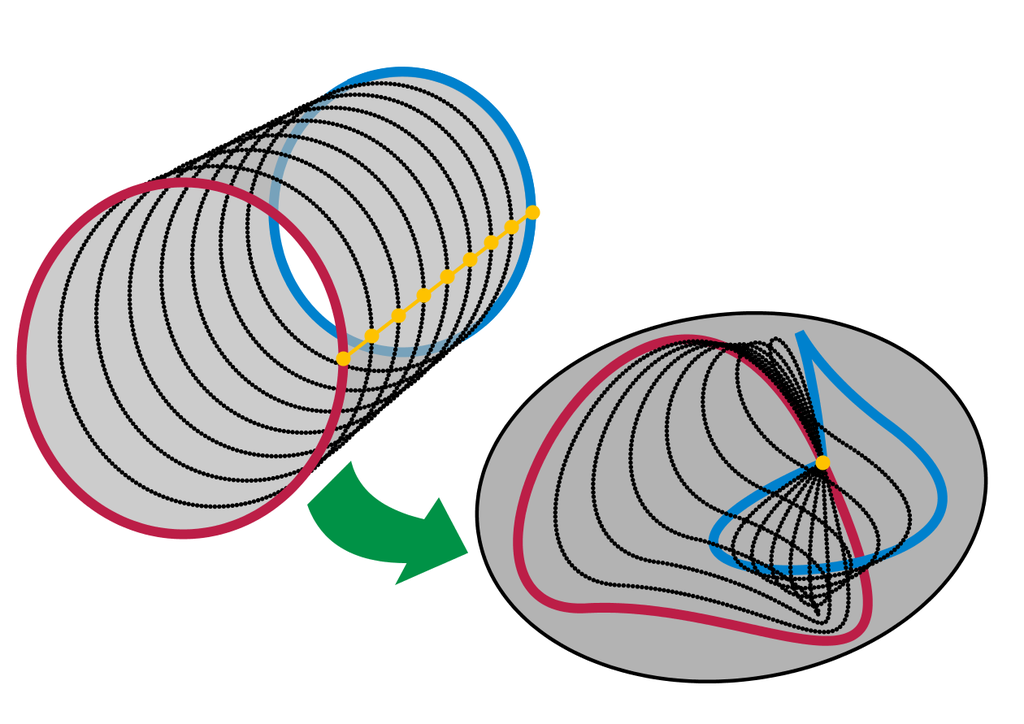
\includegraphics{homot.png}}

\renewcommand{\thesection}{\arabic{section}}
\renewcommand{\thechapter}{\sffamily\roman{chapter}}

%Otro formato para las secciones
\titleformat{\section}[block]
{\fontsize{15}{18}\bfseries\sffamily\filcenter}
{\S \thesection.}
{1em}
{}

\makeatletter
\@removefromreset{section}{chapter}
\makeatother

\begin{document}
\maketitle
\tableofcontents
\chapter{Homotopía}
\section{Homotopía: El concepto}
\begin{defn}
  Sean $(X,\TT)$ y $(Y,\TT')$ dos espacios topológicos y $f,g:X\rightarrow Y$ aplicaciones continuas. Decimos que \emph{$f$ es homótopa a $g$} si existe $F:X\times I \rightarrow Y$ continua, siendo $I=[0,1]$, que cumple
  \begin{equation*}
  \begin{cases}
    F(x,0)&=f(x) \\
    F(x,1)&=g(x) 
  \end{cases}
\end{equation*}
para todo $x \in X$. Decimos que $F$ es una \emph{homotopía entre $f$ y $g$} y lo denotamos por  $f\sim_F g$ o simplemente $f\sim g$.
    
\end{defn}

\begin{obs}
  Nótese que, para cada $t\in I$, la aplicación $F_t=F(\bullet,t):X\rightarrow Y$ es continua, que $F_0= f$ y que $F_1 = g$.
\end{obs}

  A partir de ahora , cuando no haya lugar a confusión  omitiremos escribir la topología y denotaremos un espacio topológico $(X,\TT)$ simplemente por $X$.
  \begin{prop}\label{equivhomot}
  Si $\mathcal{C}(X,Y)$ denota el conjunto de las aplicaciones continuas entre dos espacios topológicos $X$ e $Y$, la relación
  \begin{equation*}
    f \sim g \Leftrightarrow f \text{ es homótopa a } g
  \end{equation*}
  es una relación de equivalencia en $\mathcal{C}(X,Y)$.
\end{prop}
\begin{proof}
  Tenemos que probar que, para cualesquiera $f,g,h \in \mathcal{C}(X,Y)$,
  \begin{enumerate}[label=(\alph*)]
    \item\label{reflx} $f \sim f$,
    \item\label{simet} si $f \sim g$ entonces $g\sim f$ y
    \item\label{trans} si $f\sim g$ y $g\sim h$ entonces $f\sim h$.
  \end{enumerate}

  \ref{reflx} Definimos
  \begin{align*}
    F :X\times I&\longrightarrow Y\\ 
      (x,t) &\longmapsto f(x). 
    \end{align*}
    Entonces claramente $F(x,0)=F(x,1)=f(x)$ y, si $V\subset X$ es abierto entonces $F^{-1}(V)=V\times I\subset X\times I$ es abierto, luego $F$ es continua.

    \ref{simet} Supongamos que $f\sim g$ por medio de una función $F:X\times I \rightarrow Y$. Definimos 
    \begin{align*}
      G :X\times I&\longrightarrow Y\\ 
        (x,t) &\longmapsto F(x,1-t) 
      \end{align*}
      Ahora, dado $x\in X$, $G(x,0)=F(x,1)=g(x)$ y $G(x,1)=F(x,0)=f(x)$. Por otra parte, $G$ es continua por ser composición de continuas, en efecto, el siguiente diagrama conmuta
      \begin{center}
	\begin{tikzcd}
	  X \times I \arrow{r}{\tau} \arrow[bend left]{rr}{G} & X\times I \arrow{r}{F} & Y,	  
	\end{tikzcd}
con $\tau(x,t)=(x,1-t)$.
      \end{center}

      \ref{trans} Supongamos que $f\sim_F g$ y $g\sim_G h$. Defino
      \begin{equation*}
	H(x,t)=
	\begin{cases}
	  F(x,2t), & \ 0\leq t \leq \tfrac{1}{2} \\ 
	  G(x,2t-1), & \ \tfrac{1}{2} < t \leq 1.
	\end{cases}
      \end{equation*}
      Entonces $H(x,0)=f(x)$, $H(x,1)=h(x)$ y la aplicación es continua a trozos por composición y es continua porque «pega bien»: 
      \begin{equation*}
	H(x,\tfrac{1}{2})=F(x,1)=g(x)=G(x,0)=H(x,\tfrac{1}{2}^+).
      \end{equation*}
\end{proof}

\begin{defn}
  Dos espacios topológicos $X$, $Y$ se dicen \emph{equivalentes por homotopía} o \emph{del mismo tipo de homotopía} si existen $f:X\rightarrow Y$ y $g:Y\rightarrow X$ continuas tales que $g\circ f \sim \id_X$ y $f\circ g \sim \id_Y$. A las aplicaciones $f$ y $g$ se les denomina \emph{equivalencias de homotopía entre $X$ e $Y$}.
\end{defn}

\section{Homotopía relativa y retractos}
\begin{defn}[Homotopía relativa]
  Sean $X,Y$ espacios topológicos, $Z \subset X$ y $f,g:X\rightarrow Y$ aplicaciones continuas. Se dice que \emph{$f$ es homótopa a $g$ relativamente a $Z$} y se denota $f\sim_Z g$ si existe una homotopía $F$ entre $f$ y $g$ tal que $F_t|_Z = f|_Z$ para todo $t\in I$.	
\end{defn}
\begin{obs}
  En particular esto nos dice también que $f|_Z= g|_Z$. 
\end{obs}

Es un ejercicio sencillo comprobar que la homotopía relativa induce también una relación de equivalencia, de forma similar a la de la proposición \ref{equivhomot}.

\begin{defn}
  Un espacio topológico $X$ se dice \emph{contractible} si la identidad $\id_X$ es homotópica a una aplicación constante $\cc_x$ para algún $x \in X$.
\end{defn}

\begin{ejemplo}\label{rcontract}
  $\RR^n$ (con la topología usual\footnote{Decimos \emph{topología usual} de $\RR^n$ a la topología inducida por la distancia euclídea. De aquí en adelante, cuando consideremos $\RR^n$ o algún subconjunto suyo, si no se especifica, siempre se considera la topología usual o la inducida por ésta al pasar a un subconjunto.}) es contractible. En efecto, basta tomar
  \begin{align*}
    F :\RR^n\times I&\longrightarrow \RR^n\\ 
      \left( x,t \right) &\longmapsto (1-t)x. 
    \end{align*}
    Entonces $F_0=\id_{\RR^n}(x)$ y $F_1=\cc_0$, luego $\id_{\RR^n}\sim_F \cc_0$.
\end{ejemplo}

\begin{obs}
  Si un espacio topológico $X$ es contractible, entonces tiene el tipo de homotopía de un punto. En efecto, tomo $x\in X$, $\cc_x:X\rightarrow \left\{ x \right\}$ y $i:\left\{ x \right\}\hookrightarrow X$. Claramente $i\circ \cc_x=\cc_x\sim \id_X$ y $\cc_x \circ i=\id_{\left\{ x \right\}}$.
\end{obs}
\begin{defn}
  Sean $X$ un espacio topológico y $A\subset X$. Decimos que \emph{$A$ es un retracto de $X$} si existe una función $r:X\rightarrow A$ continua tal que $r|_A=\id_A$. Esta $r$ se denomina una \emph{retracción de $X$ a $A$}.
\end{defn}

\begin{ejemplo}\leavevmode
  \begin{enumerate}
    \item La esfera $S^{n-1}$ es un retracto del disco perforado $D^n-\left\{ 0 \right\}$. En efecto, la aplicación
  \begin{align*}
    r :D^n-\left\{ 0 \right\}&\longrightarrow S^{n-1}\\ 
    x &\longmapsto \frac{x}{||x||} 
    \end{align*}
    es claramente una retracción de $D^n$ a $S^{n-1}$.

  \item Si $n>m$, la aplicación
    $ r(x_1,\dots,x_n) = (x_1,\dots,x_m,0,\dots,0) $
      es una retracción de $\RR^n$ a $\RR^m$ (visto como subconjunto de $\RR^n$).
  \end{enumerate}
\end{ejemplo}

\begin{defn}
  Sea $X$ un espacio topológico y $A\subset X$. Decimos que \emph{$A$ es un retracto por deformación de $X$} si existe una homotopía $r:X\times I \rightarrow X$ tal que $r_0=\id_X$, $r_1|_A=\id_A$ y $r_1(x)\in A$ para todo $x\in X$. Es decir, $r_0$ es la identidad y $r_1$ es una retracción a $A$. Además, decimos que $A$ es un retracto por deformación \emph{fuerte} de $X$ si $r_t|_A=\id_A$ para todo $t\in I$. Esta homotopía $r$ se denomina una \emph{retracción de deformación (fuerte) de $X$ a $A$}.
\end{defn}

\begin{prop}
  Si $X$ es un espacio topológico y $A\subset X$ es un retracto por deformación de $X$, entonces $X$ tiene el mismo tipo de homotopía que $A$.
\end{prop}
\begin{proof}
  Si $r$ es la retracción de deformación de $X$ a $A$ basta considerar $r_1:X\rightarrow A$ y la inclusión $i:A\hookrightarrow X$. Ahora $r_1\circ i=r_1|_{A}=\id_A$ y $i\circ r_1 = r_1 \sim_r \id_X$. Por tanto, $r_1$ es una equivalencia de homotopía.
\end{proof}

\begin{ejemplo}\label{perforado}
  El disco perforado $D^n-\left\{ 0 \right\}$ es del mismo tipo de homotopía que la esfera $S^{n-1}$. En efecto, la aplicación
  \begin{align*}
    r_t :D^n-\left\{ 0 \right\}&\longrightarrow S^{n-1}\\ 
    x &\longmapsto (1-t)x + t\frac{x}{||x||} 
    \end{align*}
    es una retracción de deformación de $D^n$ a $S^{n-1}$ ya que $r_0=\id_{D^n}$, $r_1|_{S^{n-1}}=\id_{S^{n-1}}$ y $r_1(x)\in S^{n-1}$ para todo $x \in D^n$.
\end{ejemplo}

\section{Homotopía de caminos}
\begin{defn}
  Sea $X$ un espacio topológico. Dos caminos $\sigma$ y $\tau$ en $X$ se dicen \emph{homotópicos} si las funciones $\sigma, \tau: I \rightarrow X$ son homótopas relativamente al conjunto $\left\{ 0,1 \right\}$. Esto es, si existe una función continua $F:I\times I \rightarrow X$ tal que $F_0=\sigma$, $F_1=\tau$ y $F_t(0)=\sigma(0)=\tau(0)$, $F_t(1)=\sigma(1)=\tau(1)$, para todo $t \in I$.
\end{defn}

\begin{defn}
  Sean $X$ un espacio topológico y $x\in X$ un punto. Un \emph{lazo en $X$ con punto base $x$} es un camino $\sigma:I\rightarrow X$ tal que $\sigma(0)=\sigma(1)=x$. El conjunto de todos los lazos de $X$ con punto base $x$ se denota por $\Omega_x(X)$.
\end{defn}
\begin{obs}
  Equivalentemente, un lazo es una aplicación $\tilde\sigma:S^1\rightarrow X$ con $\tilde\sigma(1)=x$. Podemos pasar fácilmente de una definición a otra por el diagrama
      \begin{center}
	\begin{tikzcd}
	  I \arrow{r}{\exp} \arrow[bend left]{rr}{\sigma} & S^1 \arrow{r}{\tilde\sigma} & X,	  
	\end{tikzcd}
	con $\exp(t)=e^{i2\pi t}$.
      \end{center}
\end{obs}

\begin{defn}
  Sean $X$ un espacio topológico y $\sigma, \tau$ dos caminos en $X$ tales que $\sigma(1)=\tau(0)$. Se define la \emph{composición} o \emph{concatenación} de dos caminos en $X$ como el camino $\sigma * \tau: I \rightarrow X$ dado por
  \begin{equation*}
    (\sigma * \tau)(s)=
    \begin{cases}
      \sigma(2s) & \ 0\leq s\leq \tfrac{1}{2} \\
      \tau(2s-1) & \ \tfrac{1}{2} \leq s \leq 1,
    \end{cases}
  \end{equation*}
  que claramente es continuo y está bien definido.
\end{defn}

\section{Grupo fundamental}
\begin{thm}[Grupo fundamental]
  Sean $X$ un espacio topológico y $x\in X$ un punto. Consideramos en $\Omega_x(X)$ la relación de equivalencia 
  \begin{equation*}
    \sigma \sim \tau \Leftrightarrow \sigma \text{ es homotópico a } \tau,
  \end{equation*}
y el conjunto cociente por esta relación de equivalencia
\begin{equation*}
  \pi_1(X,x)=\Omega_x(X)/\sim.
\end{equation*}
Consideramos también la aplicación 
\begin{align*}
   \pi_1(X,x)\times \pi_1(X,x)&\longrightarrow \pi_1(X,x)\\ 
   ([\sigma],[\tau]) &\longmapsto [\sigma][\tau]=[\sigma * \tau]. 
  \end{align*}
  Entonces esta aplicación está bien definida e induce una estructura de grupo en $\gf(X,x)$. Este grupo se denomina el \emph{grupo fundamental de $X$ en $x$}. El grupo fundamental también recibe el nombre de \emph{primer grupo de homotopía} o \emph{grupo de Poincaré}.
\end{thm}
\begin{proof}
  Tenemos que demostrar las siguientes propiedades:
  \begin{enumerate}[label=(\alph*)]
    \item\label{biendef} \textbf{Bien definida}: Si $\sigma\sim\sigma'$ y $\tau \sim \tau'$ entonces $\sigma'*\tau'\sim \sigma * \tau$. 
    \item\label{asoc} \textbf{Asociativa}: Para cualesquiera $[\sigma],[\tau],[\gamma] \in \gf(X,x)$, $([\sigma][\tau])[\gamma]=[\sigma]([\tau][\gamma])$.
    \item\label{neutro} \textbf{Elemento neutro}: Existe un $e \in \gf(X,x)$ tal que $e[\sigma]=[\sigma]e=[\sigma]$.
    \item\label{inverso} \textbf{Elemento inverso}: Para todo $[\sigma]\in \gf(X,x)$ existe un $[\sigma]^{-1} \in \gf(X,x)$ tal que $[\sigma]^{-1}[\sigma]=[\sigma][\sigma]^{-1}=e$.
  \end{enumerate}

  \ref{biendef} \textbf{Bien definida}. Sea $F$ una homotopía entre $\sigma$ y $\sigma'$ y sea $G$ una homotopía entre $\tau$ y $\tau'$. Para $t \in I$ definimos
  \begin{equation*}
    H_t(s)=
    \begin{cases}
      F_t(2s), & \ 0\leq s\leq \tfrac{1}{2} \\
      G_t(2s-1), & \ \tfrac{1}{2} < s \leq 1,
    \end{cases}
  \end{equation*}
  que es continua ya que
  \begin{equation*}
    H_t\left(\tfrac{1}{2}\right)=F_t(1)=x=G_t(0)=H_t\left(\tfrac{1}{2}^+\right). 
  \end{equation*}
  Ahora, 
  \begin{equation*}
    H_0(s)=
    \begin{cases}
      \sigma(2s), & \ 0\leq s \leq \tfrac{1}{2} \\
      \tau (2s-1), & \ \tfrac{1}{2} < s \leq 1,
    \end{cases}
  \end{equation*}
  luego $H_0=\sigma*\tau$ y 
  \begin{equation*}
    H_1(s)=
    \begin{cases}
      \sigma'(2s), & \ 0\leq s \leq \tfrac{1}{2} \\
      \tau' (2s-1), & \ \tfrac{1}{2} < s \leq 1,
    \end{cases}
  \end{equation*}
  luego $H_1=\sigma'*\tau'$. Por tanto, $\sigma'*\tau' \sim_H \sigma*\tau$.

  \ref{asoc} \textbf{Asociativa}.
  
  \ref{neutro} \textbf{Elemento neutro}. Vamos a comprobar que el elemento neutro es $e=[\cc_x]$.

  \ref{inverso} \textbf{Elemento inverso}. Vamos a comprobar que, dado $[\sigma]\in \gf(X,x)$, el elemento inverso de $[\sigma]$ es $[\sigma]^{-1}=[\cev{\sigma}]$, con $\cev{\sigma}$ definido\footnote{ Claramente, esta definición de $\cev{\gamma}$ como el camino $\gamma$ «recorrido en sentido contrario» es válida para cualquier camino $\gamma$, no solo para lazos.} como
  \begin{equation*}
    \cev{\sigma}(s)=\sigma(1-s),
  \end{equation*}
  para cada $s \in I$.
\end{proof}
\begin{prop}\label{fstar}
  Sean $X$ e $Y$ espacios topológicos y una función continua $f:X\rightarrow Y$. Entonces $f$ induce un homomorfismo de grupos $f_*:\gf(X,x)\rightarrow \gf(Y,f(x))$ para cada $x \in X$.
\end{prop}
\begin{proof}
  Consideramos la aplicación
  \begin{align*}
    f_* :\gf(X,x)&\longrightarrow \gf(Y,f(x))\\ 
    [\sigma] &\longmapsto [f\circ \sigma],
    \end{align*}
    basta ver que $f_*$ está bien definida y es un homomorfismo de grupos.

    \textbf{Bien definida}. Sean dos lazos $\sigma$ y $\sigma'$ homotópicos por una función $F$. Consideramos la función $H=f\circ F$, $H_0=f\circ \sigma$, $H_1=f \circ \sigma'$ y $H_t(0)=f\circ\sigma(0)=f\circ\sigma'(0)$. Luego $f\circ \sigma \sim f \circ \sigma'$.

    \textbf{Homomorfismo}. Basta ver que 
    \begin{equation*}
      f\circ(\sigma*\tau (s))=
      \begin{cases}
	f(\sigma(2s)) & \ 0\leq s \leq \tfrac{1}{2} \\
	f(\tau(2s-1)) & \ \tfrac{1}{2} < s \leq 1.
      \end{cases}
    \end{equation*}
    De modo que $f\circ(\sigma*\tau)=(f\circ \sigma)*(f\circ \tau)$. Por tanto
    \begin{equation*}
      f_*([\sigma * \tau])=[f\circ(\sigma*\tau)]=[f\circ \sigma][f\circ \tau]=f_*[\sigma]f_*[\tau].
    \end{equation*}
    Luego $f_*$ es homomorfismo de grupos.
\end{proof}

\begin{prop}\label{funtgf}
  Sean $X,Y,Z$ espacios topológicos y dos funciones continuas $f:X\rightarrow Y$, $g:Y\rightarrow Z$. Entonces $(g\circ f)_*=g_*\circ f_*$.
\end{prop}
\begin{proof}
  Claramente \[(g\circ f)_*[\sigma]=[g\circ f \circ \sigma]=[g\circ(f \circ \sigma)]=g_*[f\circ \sigma]=g_* (f_* [\sigma])=(g_* \circ f_*) [\sigma].\]
\end{proof}
\begin{obs}
  Nótese que, trivialmente $(\id_{X})_*=\id_{\gf(X,x)}$.
\end{obs}
\begin{corol}
  Si $f:X\rightarrow Y$ es un homeomorfismo entre dos espacios topológicos $X$ e $Y$, entonces, para todo $x\in X$, $f_*$ es un isomorfismo de grupos entre $\gf(X,x)$ y $\gf(Y,f(x))$.
\end{corol}
\begin{proof}
  Si $f$ es un homeomorfismo, existe $g:Y\rightarrow X$ continua tal que el diagrama
  \begin{center}
    \begin{tikzcd}
      X \arrow{r}{f} \arrow{rd}[anchor=east]{\id_X} & Y\arrow{d}{g}\arrow{rd}{\id_Y} &       \\ 
      & X \arrow{r}{f} & Y
    \end{tikzcd}
  \end{center}
  conmuta. Por la proposición \ref{funtgf}, este diagrama induce otro diagrama
  \begin{center}
    \begin{tikzcd}
      \gf(X,x) \arrow{r}{f_*} \arrow{rd}[anchor=east]{\id_{\gf(X,x)}} & \gf(Y,f(x))\arrow{d}{g_*}\arrow{rd}{\id_{\gf(Y,f(x))}} &       \\ 
      & \gf(X,x) \arrow{r}{f} & \gf(Y,f(x)),
    \end{tikzcd}
  \end{center}
  también conmutativo, que nos dice que $f_*$ es un isomorfismo de grupos.
\end{proof}
\begin{thm}\label{isocamino}
  Sean $X$ un espacio topológico, $x_0,x_1\in X$ y $\gamma$ un camino que une $x_0$ y $x_1$ (esto es, $\gamma(0)=x_0$ y $\gamma(1)=x_1$). Entonces $\gamma$ induce un isomorfismo de grupos $\gamma_{\#}:\gf(X,x_0) \rightarrow \gf(X,x_1)$.
\end{thm}
\begin{proof}
  Basta tomar
  \begin{align*}
    \gamma_{\#} :\gf(X,x_0)&\longrightarrow \gf(X,x_1)\\ 
    [\sigma] &\longmapsto [\cev{\gamma}*\sigma*\gamma].
    \end{align*}
    Tenemos que ver que $\gamma_{\#}$ está bien definida, es homomorfismo y es isomorfismo.

    \textbf{Bien definida}. Supongamos que $\sigma$ y $\sigma'$ son dos caminos homotópicos $\sigma \sim_F \sigma'$. Construimos la homotopía
    \begin{equation*}
      G_t(s)=
      \begin{cases}
	\cev{\gamma}(3s) & \ 0\leq s \leq \tfrac{1}{3} \\
	F_t(3s-1) & \ \tfrac{1}{3} < s \leq \tfrac{2}{3} \\
	\gamma(3s-2) & \ \tfrac{2}{3} < s \leq 1.
      \end{cases}
    \end{equation*}

Claramente $G_t$ «pega bien» ya que $F_t(0)=x_0=\gamma(0)=\cev{\gamma}(1)$ y $F_t(1)=x_1=\gamma(1)$. Además, $G_0=\cev{\gamma}*\sigma*\gamma$, $G_1=\cev{\gamma}*\sigma'*\gamma$ y $G_t(0)=G_t(1)=x_1$. Por tanto, $\cev{\gamma}*\sigma*\gamma \sim_G \cev{\gamma}*\sigma'*\gamma$.

\textbf{Homomorfismo}. 
\begin{equation*}
  \gamma_{\#}([\sigma][\tau])= \gamma_{\#}[\sigma*\tau]=[\cev{\gamma}*(\sigma*\tau)*\gamma]=[(\cev{\gamma}*\sigma*\gamma)*(\cev{\gamma}*\tau*\gamma)]=\gamma_{\#}[\sigma]\gamma_{\#}[\tau].
\end{equation*}

\textbf{Isomorfismo}. Para ver que $\gamma_{\#}$ es de hecho un isomorfismo, basta hallar su inversa, que afirmamos que es $\cev{\gamma}_{\#}$.
\end{proof}

\begin{corol}
  Si $X$ es un espacio topológico conexo por caminos, para cualesquiera dos puntos $x_1,x_2 \in X$, $\gf(X,x_1)\cong\gf(X,x_2)$.
\end{corol}

Por tanto, cuando nuestro espacio topológico $X$ sea conexo por caminos, podremos hablar con propiedad del \emph{grupo fundamental de $X$}, puesto que será «el mismo» en todos los puntos. En el caso en que este grupo sea el trivial, se dice que $X$ es \emph{simplemente conexo}.

\section{Categorías y funtores}
En esta sección introducimos el formalismo de la Teoría de Categorías, que ofrece un marco muy general en el que estudiar ciertas propiedades de los objetos matemáticos. En Topología Algebraica, muchas de las ideas categóricas aparecen de forma natural y su estudio puede ayudar a entender mejor qué es lo que está pasando detrás a parte de que, una vez se coge cierta habilidad, permiten hacer ciertas demostraciones de forma más cómoda y elegante.

\begin{defn}
  Una \emph{categoría} $\cat$ consta de
  \begin{enumerate}
    \item Una colección de \emph{objetos} que denotamos por $\obj(\cat)$.
    \item Para cualesquiera dos objetos $X,Y$, una colección de flechas $X\rightarrow Y$ entre estos objetos, llamadas \emph{morfismos entre $X$ e $Y$}, que denotamos por $\cat(X,Y)$
    \item Una \emph{ley de composición}, para cualesquiera tres objetos $X,Y,Z$
      \begin{align*}
	\cat(X,Y)\times \cat(Y,Z)&\longrightarrow \cat(X,Z)\\ 
	  (f,g) &\longmapsto g\circ f, 
	\end{align*}
es decir
\begin{center}
  \begin{tikzcd}
X    \arrow{rr}{f}\arrow{rrdd}[anchor=north,rotate=-30]{g\circ f} && Y\arrow{dd}[anchor=west]{g} \\ 
     && \\
     &&Z,
   \end{tikzcd}
 \end{center}
 tal que cumple:
 \begin{enumerate}
   \item \textbf{Propiedad asociativa}: Dados morfismos $f:X\rightarrow Y$, $g:Y\rightarrow Z$ y $h:Z\rightarrow W$,
     \begin{equation*}
       (h\circ g)\circ f = h\circ(g\circ f).
     \end{equation*}
   \item \textbf{Elemento identidad}: Para todo objeto $X$ existe un morfismo $\id_X:X\rightarrow X$ tal que, si $Y$ es otro objeto, $f:X\rightarrow Y$, $g:Y\rightarrow X$, entonces
     \begin{equation*}
       \begin{cases}
	 f\circ \id_X=f, \text{ y} \\
	 \id_X\circ g=g.
       \end{cases}
     \end{equation*}
     Es decir, que el siguiente diagrama conmuta
     \begin{center}
       \begin{tikzcd}
	 Y	 \arrow{rr}{g}\arrow{rrdd}[anchor=north,rotate=-30]{g} && X\arrow{dd}[anchor=west]{\id_X} \arrow{rr}{f} && Y\\ 
	  && \\
	  &&X.\arrow{rruu}[anchor=north,rotate=30]{f}
	\end{tikzcd}
       \end{center}
 \end{enumerate}
  \end{enumerate}
\end{defn}
En general, para una categoría arbitraria $\cat$, $\obj(\cat)$ puede ser cualquier colección de objetos. En el caso especial en que $\obj(\cat)$ sea un conjunto, se dice que $\cat$ es una categoría \emph{pequeña}. De la misma manera, dados dos objetos $X,Y$, $\cat(X,Y)$ puede ser una colección arbitraria de flechas. En el caso en que $\cat(X,Y)$ sea un conjunto para cualesquiera dos objetos $X,Y$, decimos que $\cat$ es una categoría \emph{localmente pequeña}. La noción de categoría localmente pequeña nos permite hablar de categorías en un contexto más general en el que $\obj(\cat)$ no es un conjunto pero es una \emph{clase propia}, esto es, una colección de conjuntos que a su vez no es un conjunto, por ejemplo la clase universal, $\mathbf{V}$, que contiene a todos los conjuntos o la clase $\mathbf{Cn}$ formada por los números cardinales. Todas las categorías con las que vamos a trabajar durante el curso serán pequeñas o localmente pequeñas. 
\begin{defn}
  Sean $\cat$ una categoría, $X,Y$ objetos de $\cat$ y un morfismo $f:X\rightarrow Y$. Decimos que 
  \begin{itemize}
    \item $f$ es un \emph{monomorfismo} si es «cancelable por la izquierda», esto es, dados otro objeto $Z$ y dos morfismos $g,h:Z\rightarrow X$, si el diagrama
      \begin{center}
	\begin{tikzcd}
	  & X\arrow{rd}{f} &	  \\ 
Z \arrow{ru}{g} \arrow{rd}{h} & & Y \\
& X \arrow{ru}{f} &
	  
	\end{tikzcd}
      \end{center}
      conmuta, entonces $g=h$.
    \item $f$ es un \emph{epimorfismo} si es «cancelable por la derecha», esto es, dados otro objeto $Z$ y dos morfismos $g,h:Y \rightarrow Z$, si el diagrama
      \begin{center}
	\begin{tikzcd}
	  & Y\arrow{rd}{g} &	  \\ 
X \arrow{ru}{f} \arrow{rd}{f} & & Z \\
& Y \arrow{ru}{h} &
	  
	\end{tikzcd}
      \end{center}
      conmuta, entonces $g=h$.
    \item $f$ es un \emph{isomorfismo} si existe un morfismo $g:Y\rightarrow X$ tal que el diagrama
  \begin{center}
    \begin{tikzcd}
      X \arrow{r}{f} \arrow{rd}[anchor=east]{\id_X} & Y\arrow{d}{g}\arrow{rd}{\id_Y} &       \\ 
      & X \arrow{r}{f} & Y
    \end{tikzcd}
  \end{center}
  conmuta. Se puede probar que este morfismo $g$ es, de hecho, único, se denota por $f^{-1}$ y se llama morfismo \emph{inverso} de $f$. En el caso en que $Y=X$, si $f:X\rightarrow X$ es un isomorfismo se dice que $f$ es un \emph{automorfismo} de $X$. La clase de los automorfismos de $X$ se denota por $\aut(X)$.
  \end{itemize}
\end{defn}

Podría uno ahora detenerse a estudiar las relaciones entre epimorfismos, monomorfismos e isomorfismos: cuándo existen inversas por la izquierda o por la derecha, probar la unicidad de la inversa en el caso de los isomorfismos, entre otras cosas. Sin embargo, por no hacer el texto excesivamente pesado y añadir información con cero importancia para lo que viene a continuación, remitimos al texto de Peter Smith [citar] al lector interesado. Aquí, nos limitaremos a probar lo siguiente:

\begin{prop}
  Sea $\cat$ una categoría y $X,Y$ objetos de $\cat$. Si $f:X\rightarrow Y$ es un isomorfismo, entonces es epimorfismo y monomorfismo.
\end{prop}
\begin{proof}
  Sean $Z,Z'$ objetos de $\cat$ y $g_1,h_1:Z\rightarrow X$ $g_2,h_2:Y\rightarrow Z'$ morfismos. Supongamos que $f\circ g_1= f\circ h_1$ y que $g_2 \circ f = h_2 \circ f$, entonces los siguientes diagramas
  \begin{center}
    \begin{tikzcd}
      &X \arrow{dr}{f}\arrow[bend left]{drr}{\id_X} &   &   \\ 
      Z \arrow{ur}{g_1} \arrow{dr}{h_1} & & Y \arrow{r}{f^{-1}} & X \\
      & X \arrow{ur}{f}\arrow[bend right]{urr}{\id_X} & &
    \end{tikzcd}
  \end{center}
  \begin{center}
    \begin{tikzcd}
      &  &Y \arrow{dr}{g_2}    &   \\ 
      Y \arrow[bend right]{drr}{\id_Y}\arrow[bend left]{urr}{\id_Y}\arrow{r}{f^{-1}} & X \arrow{ur}{f} \arrow{dr}{f} & & Z'  \\
     &  & Y \arrow{ur}{h_2} & &
    \end{tikzcd}
  \end{center}
  conmutan. De la conmutatividad del primer diagrama tenemos $g_1=\id_X \circ g_1 = \id_X \circ h_1 = h_1$, luego $f$ es monomorfismo. Por otra parte, de la conmutatividad del segundo diagrama $g_2=g_2\circ\id_Y=h_2 \circ \id_Y=h_2$, luego $f$ es epimorfismo.
\end{proof}

\begin{defn}
  Sea $\cat$ una categoría. Dos objetos $X, Y$ de $\cat$ se dicen \emph{isomorfos}, y se denota $X\cong Y$, si existe un isomorfismo $f:X\rightarrow Y$.
\end{defn}

Podemos considerar ahora algunos ejemplos de categorías:

\begin{ejemplo}\leavevmode

  \paragraph{Conjuntos} La \emph{categoría de los conjuntos} $\mathbf{Sets}$ consta de:
  \begin{enumerate}
    \item La colección de objetos de $\mathbf{Sets}$ es $\obj(\mathbf{Sets})=\mathbf{V}$, la clase de todos los conjuntos.
    \item Dados dos conjuntos $X, Y$, la colección de morfismos entre $X$ e $Y$ es el conjunto $\prescript{X}{}Y$ de todas las aplicaciones (conjuntistas) entre $X$ e $Y$.
    \item La ley de composición es simplemente la composición como aplicaciones.
  \end{enumerate}
  Los monomorfismos en la categoría $\mathbf{Sets}$ son las aplicaciones inyectivas, mientras que los epimorfismos son las sobreyectivas. Los isomorfismos de $\mathbf{Sets}$ son las biyecciones, luego dos conjuntos son isomorfos si y sólo si son equipotentes.

  \paragraph{Espacios vectoriales} Sea $k$ un cuerpo. La \emph{categoría de los $k$-espacios vectoriales} $\mathbf{Vect}_k$ consta de:
  \begin{enumerate}
    \item La colección de objetos de $\mathbf{Vect}_k$ es la clase de todos los espacios vectoriales sobre $k$.
    \item Dados dos $k$-espacios vectoriales $V, V'$, la colección de morfismos entre $V$ y $V'$ es el conjunto de las aplicaciones lineales entre $V$ y $V'$.
    \item La ley de composición es simplemente la composición como aplicaciones.
  \end{enumerate}

  \paragraph{Grupos} La \emph{categoría de los grupos} $\grp$ consta de:
  \begin{enumerate}
    \item La colección de objetos de $\grp$ es la clase de todos los grupos.
    \item Dados dos grupos $G, H$, la colección de morfismos entre $G$ y $H$ es el conjunto $\mathrm{Hom}(G,H)$ de los homomorfismos de grupos entre $G$ y $H$.
    \item La ley de composición es simplemente la composición como aplicaciones.
  \end{enumerate}

  \paragraph{Espacios topológicos} La \emph{categoría de los espacios topológicos} $\top$ consta de:
  \begin{enumerate}
    \item La colección de objetos de $\top$ es la clase de todos los espacios topológicos.
    \item Dados dos espacios topológicos $X, Y$, la colección de morfismos entre $X$ e $Y$ es el conjunto $\mathcal{C}(X,Y)$ de las aplicaciones continuas entre $X$ e $Y$.
    \item La ley de composición es simplemente la composición como aplicaciones.
  \end{enumerate}
  En este caso, los isomorfismos de $\top$ serán precisamente los homeomorfismos. De esta forma podemos definir también la categoría $\top_*$ de los \emph{espacios topológicos punteados}, cuyos objetos son los pares $(X,x)$, donde $X$ es un espacio topológico y $x\in X$ y los morfismos entre $(X,x)$ e $(Y,y)$ son las aplicaciones continuas $f:X\rightarrow Y$ tales que $f(x)=y$.

  \paragraph{Homotopía} La \emph{categoría de homotopía} $\htop$ consta de:
  \begin{enumerate}
    \item La colección de objetos de $\top$ es la clase de todos los espacios topológicos.
    \item Dados dos espacios topológicos $X, Y$, la colección de morfismos entre $X$ e $Y$ es el conjunto $\mathcal{C}(X,Y)/\sim$, donde $\sim$ es la relación de equivalencia dada por la homotopía entre funciones.
    \item La ley de composición es simplemente la composición como aplicaciones.
  \end{enumerate}
  Los isomorfismos de $\htop$ son las equivalencias de homotopía. De forma análoga a la anterior, podemos considerar la categoría de homotopía \emph{con punto base} $\htop_*$, cuyos objetos son los pares $(X,x)$, donde $X$ es un espacio topológico y $x\in X$ y el conjunto de morfismos entre $(X,x)$ e $(Y,y)$ es $\top_*( (X,x) ,(Y,y) )/\sim$, donde $\sim$ es la relación de equivalencia dada por la homotopía entre funciones \emph{relativa a $x$}.

 

  \paragraph{Un grupo} Nótese que todas las categorías tratadas hasta ahora son localmente pequeñas. Veamos un ejemplo de categoría pequeña. Un grupo $G$ se puede ver como una categoría pequeña de la siguiente forma:
  \begin{enumerate}
    \item $\obj(G)$ consta de un solo elemento $\bullet$.
    \item Podemos representar cada elemento $g$ del grupo $G$ como una flecha
      \begin{center}
	\begin{tikzcd}
	  \bullet \arrow{r}{g} & \bullet	  
	  
	\end{tikzcd}
      \end{center}
      que es además un automorfismo, ya que tiene la flecha inversa
      \begin{center}
	\begin{tikzcd}
	  \bullet  & \bullet	  \arrow{l}{g^{-1}}
	  
	\end{tikzcd}
      \end{center}
      correspondiente al elemento inverso $g^{-1}$.
    \item La ley de composición viene dada por la operación del grupo, que, por ser $G$ un grupo, tiene la propiedad asociativa y elemento identidad $\id_{\bullet}$ que no es otra cosa que el elemento neutro $e$ del grupo.
  \end{enumerate}
\end{ejemplo}

La teoría de categorías nos permite hablar de un modo general de lo que significa un \emph{problema de clasificación}.

\begin{defn}
  Una \emph{clasificación} de una categoría $\cat$ es una colección $\mathcal{L}_{\cat}$ de objetos de $\cat$ tal que para todo objeto $X$ de $\cat$ existe uno y sólo un objeto de $\mathcal{L}_{\cat}$ tal que $X\cong Y$. 
\end{defn}

Veamos como algunos de los ejemplos anteriores admiten clasificaciones:
\begin{prop}
  El Axioma de Elección implica que existe una clasificación para $\mathbf{Sets}$ y para $\mathbf{Vect}_k$, dado un cuerpo $k$.
\end{prop}
\begin{proof}
  En efecto, el Axioma de Elección es equivalente al Principio de Buen Orden, que dice que todo conjunto admite un buen orden. Por tanto, dado un conjunto $X$, puedo tomar un buen orden $<$ de $X$. Ahora, todo conjunto bien ordenado es isomorfo (como conjunto bien ordenado) a un ordinal, lo que en particular implica que existe un ordinal $\alpha$ tal que $X$ es equipotente a $\alpha$. Basta tomar ahora el \emph{cardinal} de $X$: $|X|=\min\left\{ \alpha \in \mathbf{On} | X\right.$ es equipotente a $\left. \alpha \right\}$. Este ordinal es único y es siempre un ordinal inicial. Por tanto la clasificación de $\mathbf{Sets}$ es la clase de los cardinales $\mathcal{L}_{\mathbf{Sets}}=\mathbf{Cn}$, formada por todos los ordinales iniciales. 

  Por otro lado, el Axioma de Elección es equivalente a que todo espacio vectorial tiene una base. Por tanto, dado un espacio vectorial sobre $k$ $V$, puedo tomar una base $B\subset V$. Ahora, si $\kappa=|B|$, es fácil probar que $V$ es isomorfo a $k^{\kappa}=\prod_{\lambda < \kappa} k$ y que, si $\kappa \neq \kappa'$, $k^{\kappa}$ no es isomorfo a $k^{\kappa'}$. Por tanto, la clasificación de $\mathbf{Vect}_k$ es 
  \begin{equation*}
    \mathcal{L}_{\mathbf{Vect}_k}=\left\lbrace k^{\kappa} | \kappa \in \mathbf{Cn} \right\rbrace.
  \end{equation*}
\end{proof}

Siguiendo un poco con el formalismo categórico, podemos definir la noción de funtor, que también nos será de gran utilidad durante el curso.

\begin{defn}
  Sean $\cat_1$ y $\cat_2$ dos categorías. Un \emph{funtor} (\emph{covariante}\footnote{La definición de funtor \emph{contravariante} es análoga, solo que se pide que $F$ invierta la dirección de las flechas en vez de conservarla. Aún así, la distinción tampoco es necesaria ya que uno puede definir funtor contravariante a partir del covariante usando la noción de \emph{categoría dual u opuesta}. Un ejemplo de funtor contravariante viene dado por ejemplo por el que manda cada espacio vectorial a su dual y cada aplicación lineal a su traspuesta o por el paso a las álgebras de $k$-formas multilineales (tensores $k$ veces \emph{contravariantes}).} ) $F$ es una correspondencia de la forma:
  \begin{enumerate}
    \item A cada objeto $X$ de $\cat_1$ le asigna un objeto $FX$ de $\cat_2$.
    \item Dados dos objetos $X,Y$ de $\cat_1$, a cada morfismo $f:X\rightarrow Y$ le asigna un morfismo $Ff:FX\rightarrow FY$.
    \item Dados tres objetos $X,Y,Z$ de $\cat_1$, y dos morfismos $f:X\rightarrow Y$ y $g:Y\rightarrow Z$, $F(g\circ f)=Fg \circ Ff$, es decir, $F$ lleva diagramas conmutativos de $\cat_1$ a diagramas conmutativos de $\cat_2$ respetando la dirección de las flechas. Además, ha de cumplirse que para cualquier objeto $X$ de $\cat_1$ $F\id_X=\id_{FX}$.
  \end{enumerate}
\end{defn}

Enseguida veremos un ejemplo de funtor que usaremos a lo largo de todo el curso, pero antes demos otro ejemplo surgido de otra área de las matemáticas:

\begin{ejemplo}
  Consideremos una categoría $\cat$ cuyos objetos son los abiertos de algún espacio euclídeo (de dimensión finita) con punto base (es decir, pares $(U,x)$ con $U\subset \RR^n$ abierto, para algún $n$, y $x\in U$). Dados dos objetos $(U,x), (V,y)$ de $\cat$, $\cat(\left( U,x \right),(V,y))$ consiste en las aplicaciones diferenciables $f$ entre $U$ y $V$ tales que $f(x)=y$. Podemos definir entonces el funtor \emph{diferencial} $D:\cat \rightarrow \mathbf{Vect}_{\RR}$, que a cada $(U,x)$ con $U \subset \RR^m$ abierto y $x \in U$ lo manda a $\RR^m$ y a cada $f:U \rightarrow V$ con $V \subset \RR^n$ abierto le asigna la diferencial
  \begin{equation*}
    Df(x): \RR^m \longrightarrow \RR^n,
  \end{equation*}
  que es la aplicación lineal cuya matriz asociada es la matriz jacobiana de $f$ en $x$.
  Que $D$ preserva los diagramas conmutativos, respetando la dirección de las flechas es simplemente la regla de la cadena. De forma muy análoga podríamos definir el funtor \emph{tangente}, de la categoría de las subvariedades regulares a la de los $\RR$-espacios vectoriales.
\end{ejemplo}

Una propiedad interesante de los funtores es que preservan los isomorfismos. Esta propiedad es de especial utilidad a la hora de resolver problemas de clasificación, ya que nos permite discernir si dos objetos son o no isomorfos estudiando sus imágenes por cierto funtor a alguna categoría más sencilla. Precisamente esto será lo que hagamos más adelante, cuando para distinguir las distintas superficies compactas mostremos que tienen grupo fundamental distinto.

\begin{prop}
  Sean dos categorías $\cat_1$ y $\cat_2$, dos objetos $X, Y$ de $\cat_1$ y $F$ un funtor entre $\cat_1$ y $\cat_2$. Si $f:X\rightarrow Y$ es un isomorfismo de $\cat_1(X,Y)$, entonces $Ff$ es un isomorfismo de $\cat_2(FX,FY)$. En particular, si $X\cong Y$, entonces $FX \cong FY$.
\end{prop}
\begin{proof}
  Si $f$ es isomorfismo, entonces existe $g:Y\rightarrow X$ tal que el diagrama  
  \begin{center}
    \begin{tikzcd}
      X \arrow{r}{f} \arrow{rd}[anchor=east]{\id_X} & Y\arrow{d}{g}\arrow{rd}{\id_Y} &       \\ 
      & X \arrow{r}{f} & Y
    \end{tikzcd}
  \end{center}
  conmuta. Como $F$ preserva los diagramas y $F\id_Z=\id_{FZ}$ para cualquier objeto $Z$ de $\cat_1$, el diagrama
  \begin{center}
    \begin{tikzcd}
      FX \arrow{r}{Ff} \arrow{rd}[anchor=east]{F\id_X=\id_{FX}} & FY\arrow{d}{Fg}\arrow{rd}{F\id_Y=\id_{FY}} &       \\ 
      & FX \arrow{r}{Ff} & FY
    \end{tikzcd}
  \end{center}
   conmuta, luego $Ff$ es un isomorfismo.
\end{proof}

Las limitaciones de tamaño que introdujimos sobre las categorías nos permiten considerar categorías de categorías, por ejemplo, la categoría $\mathbf{Cat}$, cuyos objetos son todas las categorías pequeñas y sus morfismos los funtores entre ellas o, análogamente $\mathbf{Cat}_*$ para las categorías localmente pequeñas. Estas consideraciones evitan las paradojas de tipo Russell, ya que, por ejemplo $\mathbf{Cat}$ y $\mathbf{Cat}_*$ no son a su vez una categoría pequeña o localmente pequeña, respectivamente.

Otra forma de evitar estas paradojas es considerando una construcción inductiva, de forma que llamaríamos 0-categoría a un conjunto, 1-categoría a una categoría formada por conjuntos cuyos morfismos sean aplicaciones entre ellos, 2-categoría a una categoría de 1-categorías con funtores entre ellas, etc. De esta manera, uno puede considerar $n$-categorías, con $n\in \mathbb{N}$. Generalizando el procedimiento inductivo podríamos definir la noción de $\omega$-categoría o incluso entes de mayor rango. Estas construcciones dan lugar a lo que se conoce como teoría de categorías \emph{superior}, más conocida por su nombre en inglés «\emph{higher category theory}».

\section{Funtorialidad del grupo fundamental}

Como ya anticipábamos antes, el grupo fundamental va a constituir para nosotros un ejemplo canónico de funtor, que manejaremos a lo largo de todo el curso.

\begin{prop}
  El grupo fundamental es un funtor de $\top_*$ en $\grp$.
\end{prop}
\begin{proof}
  A cada espacio topológico punteado $(X,x)$ $\gf$ le asigna un grupo $\gf(X,x)$. Como ya vimos en la proposición \ref{fstar}, cada $f:X\rightarrow Y$ induce un homomorfismo de grupos $f_*:\gf(X,x)\rightarrow \gf(Y,f(x))$, luego $\gf f=f_*$. La preservación de los diagramas viene garantizada por la proposición \ref{funtgf}. Además, como ya observábamos entonces, $(\id_X)_*=\id_{\gf(X,x)}$.
\end{proof}

Para continuar viendo propiedades funtoriales del grupo fundamental, observemos cómo se comporta con la homotopía.

\begin{prop}
  Sean $X,Y$ espacios topológicos, $x_0\in X$ y $f,g:X\rightarrow Y$ funciones continuas $f\sim_{\left\{x_0 \right\}}g$ y $y_0=f(x_0)=g(x_0)$. Entonces los homomorfismos $f_*,g_*:\gf(X,x_0)\rightarrow \gf(Y,y_0)$ coinciden.
\end{prop}
\begin{proof}
  Como $f\sim_{\left\{x_0 \right\}}g$ y $y_0=f(x_0)=g(x_0)$, ha de existir una $F:X\times I \rightarrow Y$ continua tal que $F_0=f$, $F_1=g$ y $F_t(x_0)=y_0$ para todo $t \in I$. Ahora, sea un lazo $\alpha$ en $X$ con punto base $x_0$. Podemos considerar la función $G_t(s)=F_t(\alpha(s))$, que cumple $G_0=f\circ \alpha$, $G_1=g \circ \alpha$ y $$G_t(0)=G_t(1)=F_t(\alpha(0))=F_t(\alpha(1))=F_t(x_0)=y_0=f(x_0)=g(x_0).$$ Luego $f\circ \alpha$ y $g \circ \alpha$ son lazos homotópicos, por tanto $f_*([\alpha])=[f\circ \alpha]=[g\circ \alpha]=g_*([\alpha])$.
\end{proof}

Cabría ahora preguntarse, si $f(x_0)\neq g(x_0)$, cuál es la relación que existe entre $f_*$ y $g_*$. 

\begin{thm}[Invariancia por homotopía del grupo fundamental]
  Sean $X,Y$ espacios topológicos y $f,g:X\rightarrow Y$ dos aplicaciones continuas homotópicas. Si fijamos $x_0\in X$, existe un isomorfismo de grupos $\psi:\gf(Y,f(x_0)) \rightarrow \gf(Y,g(x_0))$ que hace el siguiente diagrama conmutativo
  \begin{center}
    \begin{tikzcd}
\gf(X,x_0)      \arrow{rr}{f_*}\arrow{rrdd}[anchor=north,rotate=-30]{g_*} && \gf(Y,f(x_0)) \arrow{dd}[anchor=west]{\psi} \\ 
       && \\
       &&\gf(Y,g(x_0)).
     \end{tikzcd}
   \end{center}
\end{thm}
\begin{proof}
  Sea $F$ la homotopía entre $f$ y $g$. Consideremos el camino dado por $\gamma(t)=F_t(x_0)$, con $t\in I$. Claramente $\gamma$ une $f(x_0)$ con $g(x_0)$, luego nuestro candidato a isomorfismo será $\psi=\gamma_{\#}$, el isomorfismo asociado al camino $\gamma$ según lo visto en el teorema \ref{isocamino}. 

Tomamos un lazo $\alpha$ en $X$ entonces es posible construir una homotopía de lazos entre $g\circ \alpha$ y $\cev{\gamma}*(f\circ \alpha)*\gamma$. Entonces, 
  \begin{equation*}
    \gamma_{\#}(f_*[\alpha])=[\cev{\gamma}*(f\circ \alpha)*\gamma]=[g\circ \alpha]=g_*[\alpha].
  \end{equation*}
  Por tanto, $\gamma_{\#}f_*=g_*$.

  La homotopía que buscamos es exactamente
  \begin{equation*}
    G_t(s)=
    \begin{cases}
      g(x_0) & t\geq3s, s\leq\tfrac{1}{3} \\
      F_{1-3s+t}(x_0) & t \leq3s, s\leq \tfrac{1}{3}\\
      F_{t}(\alpha(3s-1)) & \tfrac{1}{3} \leq s \leq \tfrac{2}{3} \\
      F_{3s-2+t}(x_0) & t\leq -3s+t, \tfrac{2}{3} \leq s \leq 1 \\
      g(x_0) & t\geq -3s+3.
    \end{cases}
  \end{equation*}
  Es fácil comprobar que esta homotopía está bien definida, es continua y es la que necesitamos.
\end{proof}

\begin{corol}
  El grupo fundamental es un funtor de $\htop_*$ en $\grp$. En particular, si $f:X\rightarrow Y$  es una equivalencia de homotopía, $\gf(X,x_0)$ y $\gf(Y,f(x_0))$ son isomorfos para cualquier $x_0 \in X$.
\end{corol}
Este resultado tiene un par de consecuencias inmediatas, muy útiles para calcular grupos fundamentales:
\begin{corol}\leavevmode
\begin{enumerate}
  \item Si $X$ es un espacio topológico contractible, entonces es simplemente conexo.
  \item Si $A$ es retracto por deformación de un espacio topológico $X$, entonces $\gf(X,a)\cong\gf(A,a)$ para todo $a\in A$.
\end{enumerate}
\end{corol}

\begin{ejemplo}\leavevmode
  \begin{enumerate}
    \item El espacio euclídeo $\RR^n$ es simplemente conexo para todo $n$. En efecto, como ya vimos en el ejemplo \ref{rcontract}, $\RR^n$ es contractible, luego por el resultado anterior, es simplemente conexo.
    \item A consecuencia del ejemplo \ref{perforado}, el disco perforado $D^n-\left\{ 0 \right\}$ tiene el mismo grupo fundamental que la esfera $S^{n-1}$.
  \end{enumerate}
\end{ejemplo}

En los siguientes capítulos continuaremos el formalismo de la homotopía y el grupo fundamental, mediante el estudio de los espacios recubridores. Esta teoría nos proporcionará una base sólida de herramientas para calcular grupos fundamentales de una cantidad diversa de espacios topológicos.

\chapter{Cubiertas}
\section{Cubiertas: Definición y ejemplos}
\begin{defn}
  Un \emph{espacio recubridor} o \emph{cubierta} de un espacio topológico $X$ es un par $(\XX,p)$, donde $\XX$ es un espacio topológico y $p:\XX\rightarrow X$ es una aplicación continua, que llamamos \emph{proyección recubridora}, que cumple:
  \begin{enumerate}
    \item $p$ es sobreyectiva y
    \item existe un recubrimiento abierto $\mathcal{U}$ de $X$ tal que, para cada $U\in \mathcal{U}$, $p^{-1}(U)=\bigsqcup_{\alpha}\tilde{U}^{\alpha}$ es unión disjunta de una familia de abiertos $\{\tilde{U}^{\alpha}\}$ que verifican que $p|_{\tilde{U}^{\alpha}}:\tilde{U}^{\alpha}\rightarrow U$ es un homeomorfismo.
  \end{enumerate}

  Los abiertos $U\in \mathcal{U}$ se llaman \emph{abiertos elementales} y los $\tilde{U}^{\alpha}$ se llaman \emph{hojas de $U$}. Dado un punto $x\in X$, el conjunto $F_x=p^{-1}(x)$ se llama \emph{fibra de $x$} y los puntos $y\in F_x$ se dice que \emph{están sobre $x$}.
\end{defn}

\begin{ejemplo}\leavevmode
  \begin{enumerate}
    \item El ejemplo más sencillo que podemos considerar es el siguiente. Dado un espacio topológico $X$ consideramos $\XX=X\times Y$ donde $Y$ es un conjunto cualquiera con la topología discreta. Si tomamos 
      \begin{align*}
	p :\XX&\longrightarrow X\\ 
	  (x,y) &\longmapsto x,
	\end{align*}
	claramente $(\XX,p)$ es una cubierta de $X$. En este caso $\mathcal{U}$ es simplemente $X$, ya que $p^{-1}(X)=\bigcup_{y\in Y}X\times\left\{ y \right\}$ y cada uno de estos es homeomorfo a $X$. La fibra de un punto $x\in X$ será simplemente $F_x=\{x\}\times Y$.
      \item Si consideramos la aplicación
	\begin{align*}
	  \exp :\RR&\longrightarrow S^1\\ 
	  t &\longmapsto e^{i2\pi t}. 
	  \end{align*}
	  Entonces $(\RR,\exp)$ es cubierta de $S^1$. Como abiertos elementales podemos tomar $U=S^1-\left\{ 1 \right\}$ y $V=S^1-\left\{ -1 \right\}$, con hojas $\exp^{-1}(U)=\bigcup_{n\in \ZZ}(n,n+1)$ y $\exp^{-1}(V)=\bigcup_{n\in \ZZ}(\tfrac{2n+1}{2},\tfrac{2n+1}{2}+1)$. 
	\item Podemos dar una cubierta de $S^1$ por $S^1$ mediante la aplicación 
	  \begin{align*}
	    p :S^1&\longrightarrow S^1\\ 
	      z &\longmapsto z^k. 
	    \end{align*}
	    De nuevo, como abiertos elementales nos valen los $U$ y $V$ del ejemplo anterior, sin embargo ahora cada uno de ellos tendrá una cantidad finita de hojas.
	  \item Podemos dar una cubierta del espacio proyectivo real $\RR P^n$ mediante la proyección canónica resultante de considerar $\RR P^n$ como $S^n$ identificado por la relación de equivalencia   \begin{equation*}
	      x\sim y \Leftrightarrow x=\pm y .
	    \end{equation*}
  \end{enumerate}
\end{ejemplo}

Para terminar la sección veamos una propiedad inmediata de las cubiertas.

\begin{prop}
  Dada una cubierta $(\XX,p)$ de un espacio topológico $X$, $p$ es un homeomorfismo local y una identificación. En particular, $X$ es un cociente topológico de $\XX$.
\end{prop}
\begin{proof}
  La demostración de que es homeomorfismo local se deduce trivialmente de la definición de cubierta. También por definición $p$ es continua y sobreyectiva. Si probamos que $p$ es abierta, habremos terminado. En efecto, tomemos $V\subset \XX$ abierto y veamos que $p(V)$ es abierto de $X$. Sea $y\in p(V)$. Entonces $y=p(x)$ para algún $x\in V$. Si tomamos $U\subset X$ un abierto elemental que contenga a $y$ y $\tilde{U}^{\alpha}$ la hoja de $U$ que contiene a $x$, entonces $x\in V\cap \tilde{U}^{\alpha}$, luego $y\in p(\tilde{U}^{\alpha}\cap V)\subset p(V)$. Como $p|_{\tilde{U}^{\alpha}}$ es un homeomorfismo, $p(\tilde{U}^{\alpha})$ es abierto de $U$ y por tanto de $X$. Es decir, dado $y\in p(V)$ hemos encontrado un entorno de $y$ contenido en $p(V)$, luego $p(V)$ es abierto.
\end{proof}

\section{Elevaciones}
\begin{defn}
Sea $(\XX,p)$ una cubierta de un espacio topológico $X$ y sea $Y$ un espacio topológico. Si $f:Y\rightarrow X$ es una aplicación continua diremos que $f$ admite una \emph{elevación} a la cubierta $(\XX,p)$ si existe una aplicación $\tilde{f}:Y\rightarrow \XX$, tal que el siguiente diagrama conmuta
  \begin{center}
    \begin{tikzcd}
      & \XX \arrow{d}{p}      \\ 
      Y \arrow{r}{f}\arrow{ru}{\tilde{f}} & X.
    \end{tikzcd}
  \end{center}
\end{defn}

\begin{prop}\label{coinciden}
  En la definición anterior, si $Y$ es conexo y Hausdorff y $\tilde{f}_1,\tilde{f}_2$ son dos elevaciones que coinciden en un punto, entonces son la misma.
\end{prop}
\begin{proof}
  Consideremos el conjunto donde ambas elevaciones coinciden
  \begin{equation*}
    H=\left\{ y\in Y | \tilde{f}_1(y)=\tilde{f}_2(y) \right\},
  \end{equation*}
  que por hipótesis es no vacío. Veamos que $H$ es abierto y cerrado en $Y$, de forma que $H=Y$ por ser $Y$ conexo.

  En efecto, tomamos $y\in H$ y llamamos $z=\tilde{f}_1(y)=\tilde{f}_2(y)$ y $x=p(z)=f(y)$. Sea $U$ un abierto elemental que contiene a $x$ y $\tilde{U}^{\alpha}$ la hoja de $U$ que contiene a $z$. Sea $W=\tilde{f}_1^{-1}(\tilde{U}^{\alpha}) \cap \tilde{f}_2^{-1}(\tilde{U}^{\alpha})\subset H$. Entonces $W$ es entorno de $y$. Si tomamos ahora otro $y'\in W$, $\tilde{f}_1(y'),\tilde{f}_2(y') \in \tilde{U}^{\alpha}$. Como $p|_{\tilde{U}^{\alpha}}$ es homeomorfismo, $\tilde{f}_1(y')=\tilde{f}_2(y')$. Por tanto, $W\subset H$, luego $H$ es abierto.
  Por otra parte, $H$ es cerrado por ser el conjunto donde coinciden dos aplicaciones continuas y ser $Y$ Hausdorff.
\end{proof}

\begin{prop}
  Sean $(\XX,p)$ una cubierta de un espacio topológico $X$ y $\gamma:I\rightarrow X$ un camino con origen $\gamma(0)=x$. Si fijamos un punto $y\in F_{x}$, entonces existe una única elevación $\tilde{\gamma}_{y}$ de $\gamma$ tal que $\tilde{\gamma}_{y}(0)=y$. 
\end{prop}

\begin{obs}
  El elevado de una concatenación de lazos $\sigma*\tau$ en un punto $y$ es $\tilde{\sigma}_y*\tilde{\tau}_{\tilde{\sigma}_y(1)}$. El elevado de un «camino inverso» $\cev{\sigma}$ es $\cev{\tilde{\sigma}}$
\end{obs}

\begin{proof}
Antes de dar la demostración necesitamos probar un lema previo.
\begin{lema}
  Sea $(K,d)$ un espacio métrico compacto, y $F:K\rightarrow X$ una aplicación continua. Sea $X=\bigcup_{\alpha}U_{\alpha}$ un recubrimiento por abiertos. Entonces existe un $\mu >0$ tal que para todo $A\subset K$ con $\mathrm{diam}(A)=\sup\left\{ d(x,y)|x,y \in A \right\}<\mu$, se tiene que existe $\alpha$ tal que $A\subset F^{-1}(U_{\alpha})$. A cualquiera de estos $\mu$ se le llama \emph{número de Lebesgue del recubrimiento $\{U_\alpha\}$ para la función $F$}.
\end{lema}

\textbf{Demostración del lema}. Supongamos que no. Entonces para cada $n\in \mathbb{N}$ existe $A_n=B(x_n,\tfrac{1}{n})\subset K$ tal que $F(A_n)$ no está contenido en ningún abierto del recubrimiento. Por la compacidad de $K$, existe una subsucesión convergente $x_{n_k}\rightarrow x_0 \in K$. Ahora, sea $\alpha_0$ tal que $F(x_0)\in U_{\alpha_0}$ y sea $\epsilon>0$ tal que $F(B(x_0,\epsilon))\subset U_{\alpha_0}$, que existe por ser $F$ continua. Para $n$ suficientemente grande, $d(x_n,x_0)<\epsilon/2$ y $1/n<\epsilon/2$. Por tanto $A_n\subset B(x_0,\epsilon)$ y $F(A_n) \subset U_{\alpha_0}$ y llegaríamos a una contradicción.

  \textbf{Existencia}. Tomamos el conjunto de abiertos elementales $\mathcal{U}=\left\{ U_{\alpha} \right\}$ y consideramos la familia $\left\{ \gamma^{-1}(U_{\alpha}) \right\}$, que es un recubrimiento por abiertos de $I$. Si tomamos $\mu$ el número de Lebesgue del recubrimiento, entonces, dados $t,s \in I$ tales que $|t-s|<\mu$, $[s,t]\subset \gamma^{-1}(U_{\beta})$ para algún $\beta$. Sea ahora una partición de $I$, $0=t_0<t_1<\cdots<t_n=1$ tal que $|t_i-t_{i+1}|<\mu$. Entonces existe un $\beta$ tal que $\gamma([0,t_1])\subset U_{\beta}$. Fijado ahora un punto $y\in F_{x}$, tomamos $\tilde{U}_{\beta}^{\alpha}$ la hoja de $U_{\beta}$ que contiene a $y$. Como $p|_{\tilde{U}_{\beta}^{\alpha}}:\tilde{U}_{\beta}^{\alpha}\rightarrow U_{\beta}$ es homeomorfismo, construyo $\tilde{\gamma}_{y}^1(t)=p|_{\tilde{U}_{\beta}^{\alpha}}^{-1}(\gamma(t))$ para $t\in[0,t_1]$. Análogamente construyo $\tilde{\gamma}_{y}^k(t)$ para $t\in[t_{k-1},t_k]$ y, finalmente $\tilde{\gamma}_{y}=\tilde{\gamma}_{y}^1*\cdots*\tilde{\gamma}_{y}^n$.

  \textbf{Unicidad}. Sea otra elevación $\bar{\gamma}_y$ de $\gamma$ con $\bar{\gamma}_y(0)=y$. Por la proposición \ref{coinciden}, como $I$ es conexo y Hausdorff y $\bar{\gamma}_y$ y $\tilde{\gamma}_y$ coinciden en un punto, tienen que ser iguales.
\end{proof}

\begin{corol}
  Si $X$ es un espacio topológico conexo por caminos y $(\XX,p)$ es una cubierta de $X$, entonces, para cualesquiera $x,y\in X$, $F_x$ y $F_y$ tienen el mismo cardinal. A este cardinal lo llamamos \emph{número de hojas} de la cubierta $(\XX,p)$.
\end{corol}
\begin{proof}
  Sea $\gamma$ un camino que une $x$ e $y$. Tomamos $\xx\in F_x$ y elevamos $\gamma$ a un camino $\tilde{\gamma}_{\xx}$, que además sabemos que es único. Como $y=\gamma(1)=p(\tilde{\gamma}_{\xx}(1))$, tenemos que $\tilde{\gamma}_{\xx}(1)\in F_y$. Esto nos da una aplicación inyectiva
  \begin{align*}
     F_x&\longrightarrow F_y\\ 
     \xx &\longmapsto \tilde{\gamma}_{\xx}(1). 
    \end{align*}
    Análogamente podemos construir una aplicación inyectiva $F_y\rightarrow F_x$. Por tanto $F_x$ es equipotente a $F_y$.
\end{proof}

\begin{corol}\label{elevhomot}
  Sean $(\XX,p)$ una cubierta de un espacio topológico $X$, $Y$ otro espacio topológico, $f:Y\rightarrow \XX$ continua y $F:I\times Y\rightarrow X$ continua con $F_0=p\circ f$. Entonces existe una única $\tilde{F}:I\times Y \rightarrow \XX$ elevación de $F$ tal que $\tilde{F}_0=f$.
\end{corol}
\begin{proof}
  Dado $y \in Y$, tomamos el camino $\gamma_y(t)=F_t(y)$ para $t\in I$. Por la proposición, existe un único levantamiento de $\gamma_y$, que llamaremos $\tilde{\gamma}_y$, que cumple $\tilde{\gamma}_y(0)=f(y)$. Podemos definir entonces $\tilde{F}_t(y)=\tilde{\gamma}_y(t)$. Claramente $\tilde{F}$ es elevación de $F$ y $\tilde{F}_0=f$. Basta ver que esta $\tilde{F}$ así construida es continua.

  Sea $(t_0,y_0)\in I \times Y$. De forma análoga a la demostración de la proposición, tomo el conjunto de abiertos elementales $\mathcal{U}=\left\{ U_{\alpha} \right\}$ y la familia $\{\gamma_{y}^{-1}(U_{\alpha})\}$, que es un recubrimiento por abiertos de $I$. Tomamos el número de Lebesgue y particionamos $I$ igual que en la demostración de la proposición, de forma que existe un $\beta$ y existe un entorno $V$ de $t_0$ tal que $F(V\times\left\{ y_0 \right\})=\gamma_{y_0}(V)\subset U_{\beta}$. Por tanto, como $F$ es continua, existe un entorno $W$ de $(t_0,y_0)$ tal que $F(W)\subset U_{\beta}$. Sea $\tilde{U}^{\alpha}_\beta$ la hoja de $U_\beta$ que contiene a $f(y)$. Ahora $p|_{\tilde{U}^{\alpha}_{\beta}}:\tilde{U}^{\alpha}_{\beta}\rightarrow U_\beta$ es homeomorfismo y, si $(t,y)\in W\subset U_{\beta}$ entonces $\tilde{F}(t,y)=\tilde{\gamma}_y(t)=p|_{\tilde{U}^{\alpha}_{\beta}}^{-1}(\gamma_y(t))$. Por tanto, $\tilde{F}$ es continua en $W$ y en particular en $(t_0,y_0)$.
\end{proof}

\section{Cubiertas y grupo fundamental}
\begin{prop}
  Sean $(\XX,p)$ una cubierta de un espacio topológico $X$ y $x\in X$. Entonces, para cualquier $\xx \in F_x$, la aplicación inducida entre grupos fundamentales $p_*:\gf(\XX,\xx)\rightarrow \gf(X,x)$ es un monomorfismo. Por tanto, $\gf(\XX,\xx)$ es isomorfo a un subgrupo $\im(p_*)<H$.
\end{prop}
\begin{proof}
  Sean dos lazos $\alpha, \beta$ en $\XX$ con punto base $\xx$. Tenemos que probar que si $p\circ \alpha \sim p\circ \beta$ entonces $\alpha \sim \beta$. En efecto, si $F$ es una homotopía entre $p\circ \alpha$ y $p\circ \beta$, podemos considerar su elevación $\tilde{F}$, única si imponemos $\tilde{F}_0=\alpha$, dada por el corolario \ref{elevhomot}, que claramente cumple $\tilde{F}_1=\beta$.
\end{proof}
\begin{prop}
  Sea $Y$ un espacio topológico conexo y localmente conexo por caminos. Sean $(\XX,p)$ una cubierta de un espacio topológico $X$ y sea $f:Y\rightarrow X$ una función continua. Fijamos $y_0\in Y$, $x=f(y_0)$ y $\xx \in F_x$. Entonces $f$ admite una elevación si y sólo si
 $\im (f_*) < \im (p_*)$.   
\end{prop}

\begin{obs}
  Si $Y$ es simplemente conexo, $f$ siempre se puede elevar.
\end{obs}

\begin{proof}
  Para ver que es condición necesaria basta ver que, si $\tilde{f}$ es una elevación de $f$,
  \begin{equation*}
    \im(f_*)=f_*(\gf(Y,y_0))=p_*(\tilde{f}_*(\gf(Y,y_0)))<p_*(\gf(\XX,\xx))=\im(p_*).
  \end{equation*}

  Veamos que también es condición suficiente. Sea $y\in Y$. Se trata de definir $\tilde{f}(y)$. Como en particular $Y$ es conexo por caminos, elegimos un camino $\sigma$ en $Y$ que une $y_0$ con $y$. Entonces, $f\circ \sigma$ es un camino en $X$ de origen $x$ y extremo $f\circ \sigma (1)=f(y)$. Elevamos $f\circ \sigma$ a un camino $\widetilde{f\circ\sigma}_{\xx}$ en $\XX$ con origen $\xx$ y definimos $\tilde{f}(y)=\widetilde{f\circ\sigma}_{\xx}(1)$. Tenemos que ver que esta $\tilde{f}$ está bien definida y es continua.

  \textbf{Bien definida}. Sea otro camino $\tau$ entre $y_0$ e $y$. Si $\tau$ es homótopo a $\sigma$ entonces $f\circ \sigma\sim f\circ \tau$, luego $\widetilde{f\circ\sigma}_{\xx}\sim\widetilde{f\circ\tau}_{\xx}$. Por tanto $\widetilde{f\circ\sigma}_{\xx}(1)=\widetilde{f\circ\tau}_{\xx}(1)$ y la $\tilde{f}(y)$ obtenida es la misma. Si $\tau$ no es homótopo a $\sigma$, consideramos $\sigma*\cev{\tau}$ lazo con punto base $y_0$. Ahora, por la hipótesis $f\circ(\sigma*\cev{\tau})=f\circ\sigma * f\circ \cev{\tau}$ es un lazo en $X$ con punto base $x=f(y_0)$. Por tanto, $\widetilde{f\circ\tau}_{\xx}(1)=\widetilde{f\circ\cev{\tau}}_{\xx}(0)=\widetilde{f\circ\sigma}_{\xx}(1)=\tilde{f}(y)$.

  \textbf{Continua}. Sean $U$ un abierto elemental que contenga a $f(y)$ y $\tilde{U}$ la hoja de $U$ que contiene a $\tilde{f}(y)$. Como $Y$ es localmente conexo por caminos y $f$ es continua, podemos tomar un entorno $V\subset Y$ de $y$ conexo por caminos tal que $f(V)\subset U$. Basta ver ahora que $\tilde{f}(V)\subset \tilde{U}$. Sea entonces un punto $y'\in V$. Tomamos un camino $\alpha$ en $V$ que une $y$ e $y'$. Entonces $\sigma * \alpha$ une $y_0$ e $y'$. Ahora, $$\tilde{f}(y')=\widetilde{f\circ(\sigma*\alpha)}_{\xx}(1)=\widetilde{f\circ\sigma}_{\xx}*\widetilde{f\circ\alpha}_{\tilde{\sigma}(x)}(1)\in \tilde{U}.$$ Ya que las elevaciones de los caminos $f\circ \sigma$ y $f\circ \alpha$ están totalmente contenidas en la hoja $\tilde{U}$ de $f(y)$.
\end{proof}

Cabría preguntarse ahora cómo se relacionan las imágenes por $p_*$ de los grupos fundamentales $\gf(\xx,\XX)$ para distintos puntos de la fibra, $\xx\in F_x$.

\begin{prop}
  Si $(\XX,p)$ es una cubierta de un espacio topológico $X$ con $\XX$ conexo por caminos, entonces, para dos puntos $y,z\in F_x$, $p_*(\gf(\XX,y))$ y $p_*(\gf(\XX,z))$ son subgrupos conjugados de $\gf(X,x)$. Además el conjunto $\bigcup_{\xx \in F_x} p_*(\gf(\XX,\xx))$ es una clase de conjugación de $\gf(X,x)$.
\end{prop}
\begin{proof}
  Como $\XX$ es conexo por caminos, puedo tomar un camino $\delta$ en $\XX$ que una $y$ y $z$. Además, como $y,z\in F_x$, $\xi=p\circ \delta$ es un lazo en $X$ con punto base $x$. Tomamos un elemento de $p_*(\gf(\XX,z))$ de la forma $p_*[\beta]$. Como $\delta$ induce un isomorfismo $\delta_\#$ entre $\gf(\XX,y)$ y $\gf(\XX,z)$, $[\beta]$ puede escribirse en la forma $[\cev{\delta}*\alpha*\delta]$, con $\alpha \in \gf(\XX,y)$. Ahora
  \begin{equation*}
    p_*[\beta]=p_*[\cev{\delta}*\alpha*\delta]=[p\circ\cev{\delta}][p\circ\alpha][p\circ\delta]=[\xi]^{-1}[p\circ\alpha][\xi]=[\xi]^{-1}(p_*[\alpha])[\xi].
  \end{equation*}
Es decir, $p_*(\gf(\XX,z))=[\xi]^{-1}p_*(\gf(\XX,y))[\xi]$, luego $p_*(\gf(\XX,y))$ y $p_*(\gf(\XX,z))$ son conjugados.

Veamos ahora que $\bigcup_{\xx \in F_x} p_*(\gf(\XX,\xx))$ es una clase de conjugación. Sean $\xx \in F_x$ y $p_*[\sigma]\in p_*(\gf(\XX,\xx))$. Dado un lazo $\xi$ en $X$ con punto base $x$, puedo elevarlo a un camino $\tilde{\xi}$ con $\tilde{\xi}(0)=\xx$. Llamando ahora $\xx'=\tilde{\xi}(1)$ resulta que $\tilde{\xi}_{\#}$ es un isomorfismo entre $\gf(\XX,\xx)$ y $\gf(\XX,\xx')$. Tenemos entonces
\begin{equation*}
  [\xi]^{-1}(p_*[\sigma])[\xi]=[p\circ \cev{\tilde{\xi}} * p\circ \sigma * p\circ \tilde{\xi}]=p_*[\cev{\tilde{\xi}}*\sigma*\tilde{\xi}]=p_*(\tilde{\xi}_{\#}[\sigma])\in p_*(\gf(\XX,\xx')).
\end{equation*}
\end{proof}

\begin{prop}
  Si $(\XX,p)$ es una cubierta de un espacio topológico $X$ y $x\in X$, entonces el grupo fundamental $\gf(X,x)$ actúa por la derecha sobre $F_x$. A cada lazo $\alpha$ en $X$ con punto base $x$ le asignamos la biyección $\xx.[\alpha]=\tilde{\alpha}_{\xx}(1)$, para $\xx \in F_x$. El estabilizador por esta acción de un punto $\xx\in F_x$ es $p_*(\gf(\XX,\xx))$.
\end{prop}
\begin{proof}
  Para ver que la aplicación $[\alpha]\rightarrow \bullet.[\alpha]$ es una acción, debemos probar que es un homomorfismo de grupos. Es decir, que dado $\xx\in \XX$, $\xx.([\alpha][\beta])=(\xx.[\alpha]).[\beta]$ y que $\xx.[\cc_x]=\xx$. Ahora,
  \begin{equation*}
    \xx.([\alpha][\beta])=\xx([\alpha*\beta])=\widetilde{\alpha*\beta}_{\xx}(1)=\tilde{\beta}_{\tilde{\alpha}_{\xx}(1)}(1)=(\xx.[\alpha]).[\beta]
  \end{equation*}
  mientras que $\xx.[\cc_x]=\tilde{\cc_x}_{\xx}(1)=\xx$.

  Por otra parte, $\xx.[\alpha]=\xx$ si y sólo si $\tilde{\alpha}_{\xx}(1)=\xx$, es decir, si $\tilde{\alpha}_{\xx}$ es un lazo en $\XX$. Ahora $[\alpha]=[p\circ \tilde{\alpha}_{\xx}]=p_*[\tilde{\alpha}_{\xx}]\in p_*(\gf(\XX,\xx))$, luego el estabilizador de $\xx$ es $p_*(\gf(\XX,\xx))$.
\end{proof}
\end{document}



